\documentclass{article}
\usepackage[T1]{fontenc}
\usepackage{lmodern}
\usepackage{amsmath}
\usepackage{graphicx}
\usepackage{float}
\usepackage{listings}
\usepackage{xcolor}
\usepackage[polish]{babel}

\usepackage[a4paper, margin=2.54cm]{geometry}

\title{Praca domowa 1\\Ryzyko empiryczne oraz \\
metoda najmniejszych kwadratów}
\author{Damian Jankowski s188597}

\begin{document}

\maketitle

\section{Wstęp}
Celem tego sprawozdania jest przedstawienie dwóch ważnych 
koncepcji w dziedzinie sztucznej inteligencji - 
wyznaczania parametrów modelu statystycznego metodą 
najmniejszych kwadratów oraz obliczania ryzyka empirycznego. 
Metoda najmniejszych kwadratów jest jedną z najpopularniejszych 
technik szacowania parametrów modelu na podstawie danych. a 
ryzyko empiryczne jest ważnym narzędziem do oceny jakości 
modelu i prognozowania jego skuteczności na nowych danych. 

Poniżej znajdują się rozwiązania przykładowych zadań z
zastosowaniem tych pojęć.

\section{Zadanie 1}
\subsection{Dane}
Mamy zbiór danych wejściowych $x$ oraz wyników oczekiwanych $d$.
\begin{center}
$
\textbf{x} = 
    \begin{bmatrix}
        -1.21 \\ 0.1 \\ 0.4 \\ 0.82
    \end{bmatrix} 
\textbf{d} = 
    \begin{bmatrix}
        2.3 \\ 3.4 \\ 5.1 \\ 6.3
    \end{bmatrix} 
$
\end{center}
Odwzorowanie jest przedstawione wzorem $y = f(x, w) = w_1x^2 + w_2x$.

\subsection{Rozwiązanie}
\subsubsection{Wyznaczenie parametrów modelu}
Parametry modelu można wyznaczyć za pomocą metody najmniejszych kwadratów.

Najpierw należy wyznaczyć równanie ryzyka empirycznego, korzystając z tego wzoru:

\begin{equation}
E_{emp}(w) = \frac{1}{n}\sum_{i=1}^n (f(x_i, w) - d_i)^2 =
\frac{1}{n}\sum_{i=1}^n (w_1x_i^2 + w_2x_i - d_i)^2
\end{equation}

\begin{equation*}
    \begin{aligned}
    E_{emp}(w) = \frac{1}{4}\Bigl(
        ((-1.21)^2w_1 - 1.21w_2 - 2.3)^2 +
        ((0.1)^2w_1 + 0.1w_2 - 3.4)^2 + \\
        ((0.4)^2w_1 + 0.4w_2 - 5.1)^2 +
        ((0.82)^2w_1 + 0.82w_2 - 6.3)^2
        \Bigr)\\
    = 0.655353w_1^2 -0.577595w_1w_2 - 4.22678w_1 +
    0.576625w_2^2 - 2.3815w_2 + 20.6575
    \end{aligned}
\end{equation*}

Następnie należy wyznaczyć pochodne cząstkowe i wyznaczyć 
minimum funkcji $E_{emp}(w)$,
czyli punkt, w którym pochodne cząstkowe są zerowe.

\begin{equation}
    \begin{aligned}
        \begin{cases}
            \cfrac{\partial E_{emp}}{\partial w_1} = 0\\
            \cfrac{\partial E_{emp}}{\partial w_2} = 0
        \end{cases}
    \end{aligned}
\end{equation}

Dla wyznaczonej funkcji $E_{emp}(w)$ otrzymujemy:

\begin{equation*}
    \begin{aligned}
        \begin{cases}
            1.31071w_1 - 0.577595w_2 - 4.22678 = 0\\
            -0.577595w_1 + 1.15325w_2 - 2.3815 = 0
        \end{cases}
    \end{aligned}
\end{equation*}

\begin{equation*}
    \begin{aligned}
        \begin{cases}
            w_1 = 5.30587682 \\
            w_2 = 4.72244169
        \end{cases}
    \end{aligned}
\end{equation*}

Wzór na funkcję $f(x, w)$ przyjmuje postać $y = f(x, w) = 5.30587682x^2 + 4.72244169x$.

\begin{figure}[H]
    \centering
    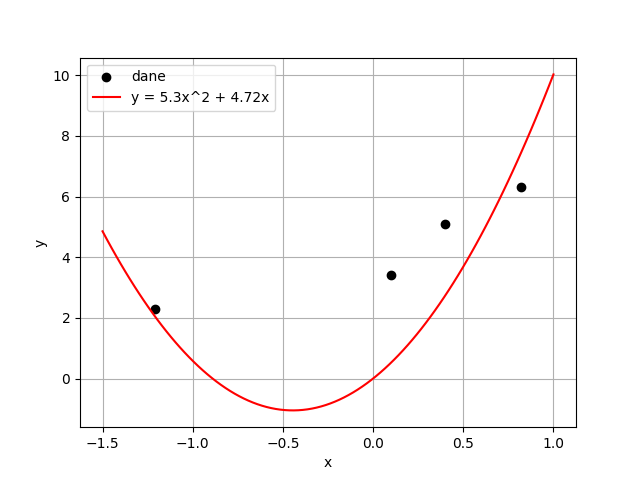
\includegraphics[width=0.5\textwidth]{plot.png}
    \caption{Wykres funkcji $f(x, w)$}
\end{figure}

\subsubsection{Obliczenie ryzyka empirycznego}
By obliczyć ryzyko empiryczne, należy podstawić do wzoru na $E_{emp}(w)$ obliczone wcześniej
wagi. 

Dla tego przykładu otrzymujemy:

\begin{equation*}
    \begin{aligned}
    E_{emp}(w) = 3.800878800281463
    \end{aligned}
\end{equation*}

\section{Zadanie 2}
\subsection{Dane}
Mamy zbiór danych wejściowych $x_1, x_2$ oraz wyników oczekiwanych $d$.
\begin{center}
$  
\textbf{x1} = 
    \begin{bmatrix}
        0.2 \\ -0.3 \\ -0.5 \\ -0.1 \\ -1.0 \\ -0.3 \\ 0.1
    \end{bmatrix} 
\textbf{x2} = 
    \begin{bmatrix}
        0.3 \\ 0.4 \\ 3.3 \\ 4.8 \\ 3.2 \\ 7.2 \\ 3.4
    \end{bmatrix} 
\textbf{d} = 
    \begin{bmatrix}
        0.8 \\ 0.2 \\ -0.3 \\ 1.2 \\ 1.6 \\ 0.5 \\ -0.2
    \end{bmatrix} 
$
\end{center}
Odwzorowanie jest przedstawione wzorem $y = f(x, w) = w_1x_1 + w_2x + w_3x_1x_2 + 
w_4x_1/x_2 +w_5x_1^2 +w_6x_2^2$.

\subsection{Rozwiązanie}
Dla podanych danych wagi wynoszą:
$
\textbf{w} = 
    \begin{bmatrix}
        w_1 \\ w_2 \\ w_3 \\ w_4 \\ w_5 \\ w_6
    \end{bmatrix}
=
    \begin{bmatrix}
        -35.50911108 \\ -1.60709009 \\ 9.83501361 \\ 11.68327077 \\ 1.78661579 \\ 0.44397207
    \end{bmatrix}
$.
Natomiast $E(w)$ wynosi $0.0306398$.

\section{Zadanie 3}
\subsection{Dane}
Dane wejściowe $x_1, x_2$ oraz $d$ są takie same jak w zadaniu 2.
Natomiast odzworowanie jest przedstawione wzorem $y = f(x, w) = w_1x_1 + w_2x + w_3x_1x_2 + w_4x_1/x_2$.

\subsection{Rozwiązanie}

Dla podanych danych wagi wynoszą:
$
\textbf{w} = 
    \begin{bmatrix}
        -2.78280549 \\  0.09515916 \\  0.45212008 \\  1.33611354
    \end{bmatrix} 
$.
Natomiast $E(w)$ wynosi $2.2706643$.

\section{Wnioski}
Metoda najmniejszych kwadratów jest prostą i szybką metodą 
estymacji parametrów modelu, która dobrze sprawdza się w 
przypadku prostych modeli.

Metoda ta ma jednak kilka wad, takich jak wrażliwość 
na odstające wartości oraz brak możliwości uwzględnienia 
zmiennych kategorycznych czy nieliniowych zależności.

W przypadku bardziej skomplikowanych modeli, gdzie zależność 
między zmiennymi jest nieliniowa, lepsze rezultaty daje 
stosowanie metod gradientowych, które pozwalają na znalezienie 
minimum funkcji kosztu w bardziej ogólnym przypadku.

Metoda gradientowa jest jednak bardziej złożona i wymaga 
większej liczby obliczeń niż metoda najmniejszych kwadratów.

W praktyce stosuje się różne metody w zależności od charakteru 
danych oraz celu modelowania.


\section{Kod programu}
\lstinputlisting[
language=python,  
basicstyle=\small\tt,
keywordstyle=\color{blue},
backgroundcolor=\color{cyan!10}
]{main.py}

\end{document}
